\chapter{Jet Results and Outlook} \label{ch:cando}

\section{8 TeV Inclusive Jet Results and Discussion}

\subsubsection{Differential Jet Cross-Section}

\afterpage{%

\begin{figure}
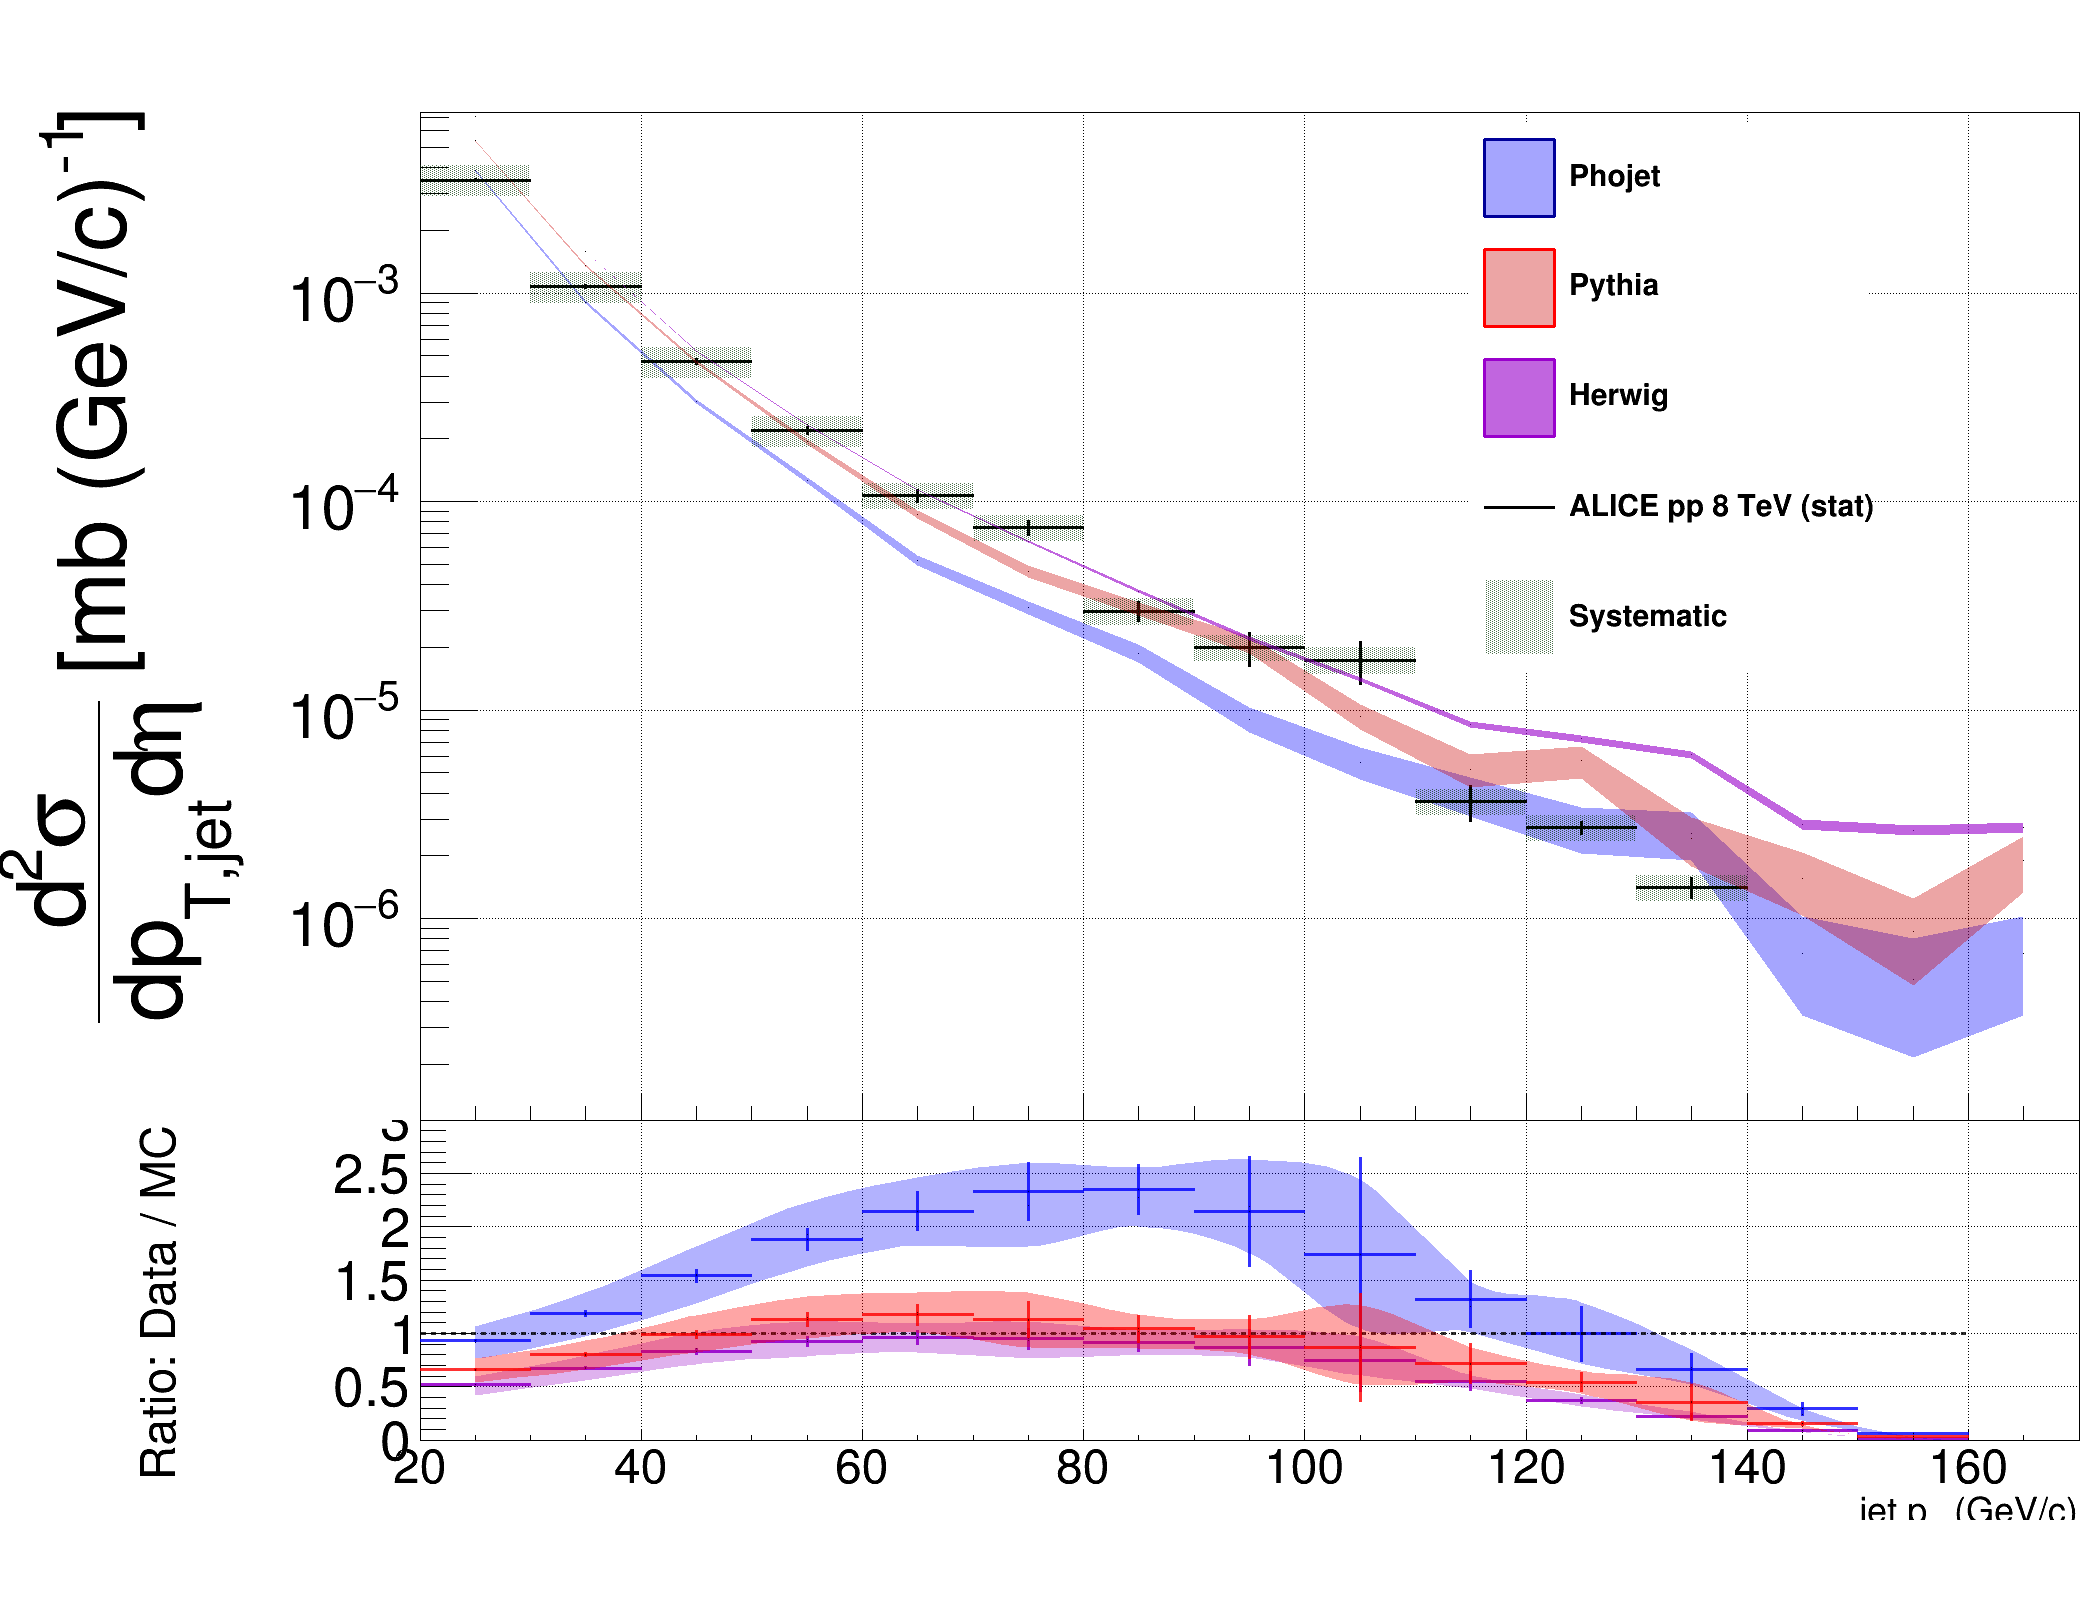
\includegraphics[width=\linewidth]{XSecR02}
\centering
\caption{8 TeV inclusive jet differential cross-section for R = 0.2.}
\label{fig:JetXsecR02}
\end{figure}

\begin{figure}
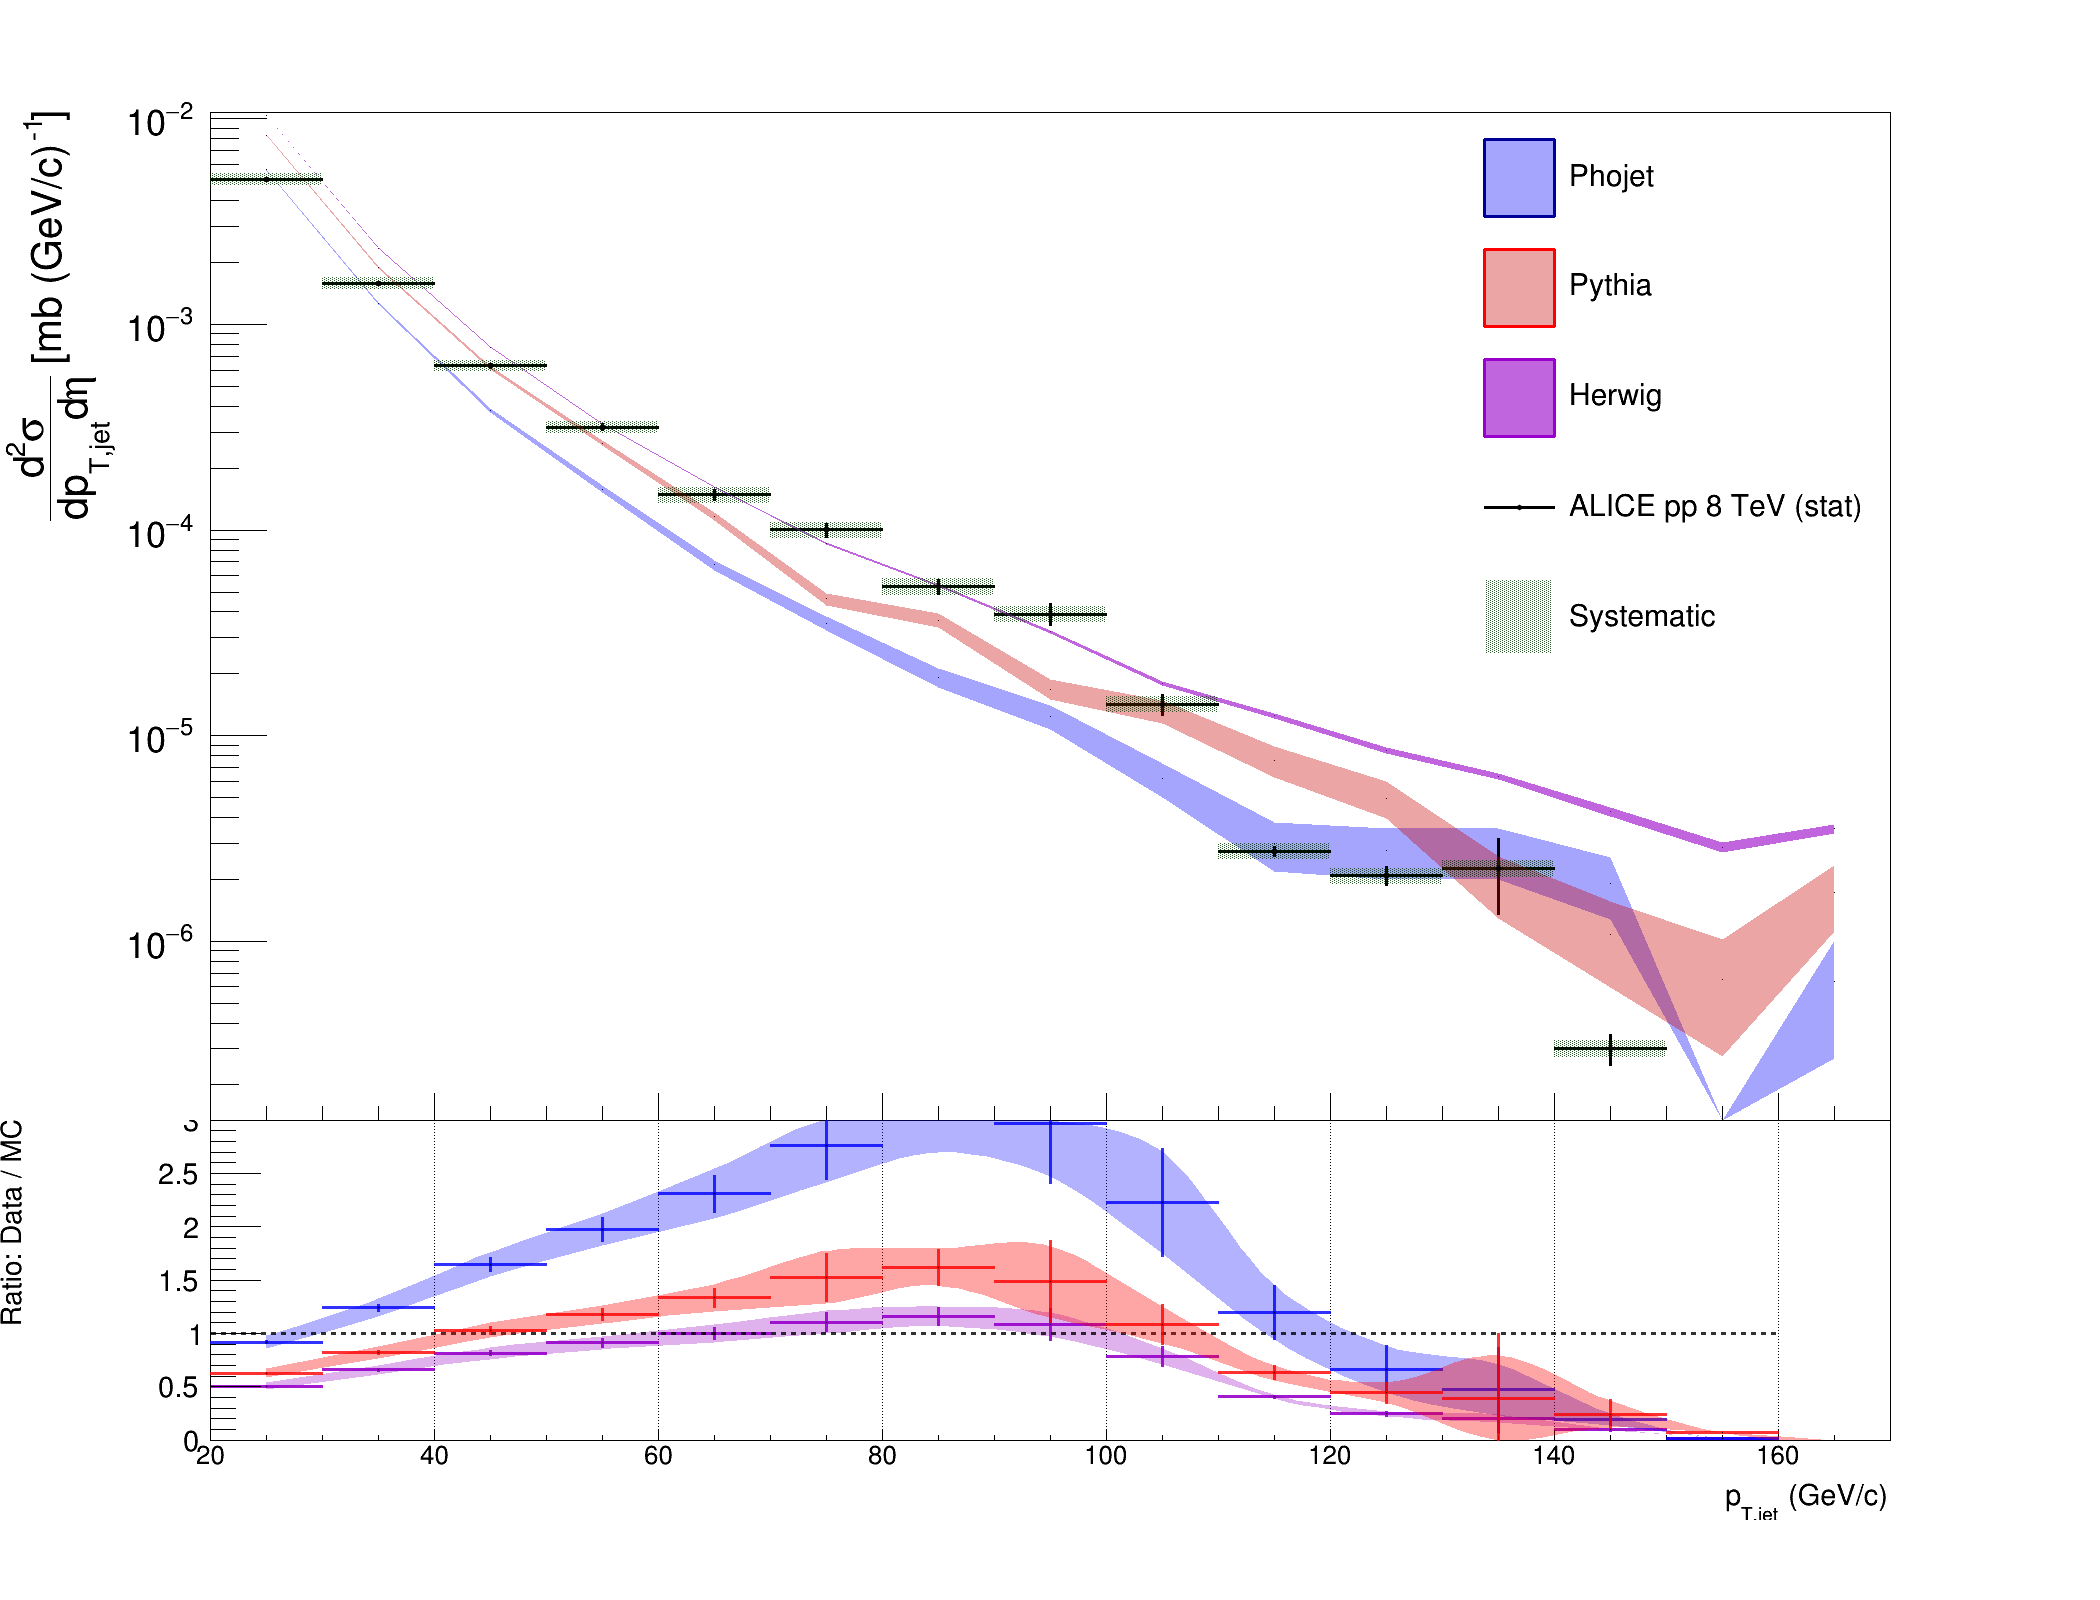
\includegraphics[width=\linewidth]{XSecR03}
\centering
\caption{8 TeV inclusive jet differential cross-section for R = 0.3.}
\label{fig:JetXsecR03}
\end{figure}

\begin{figure}
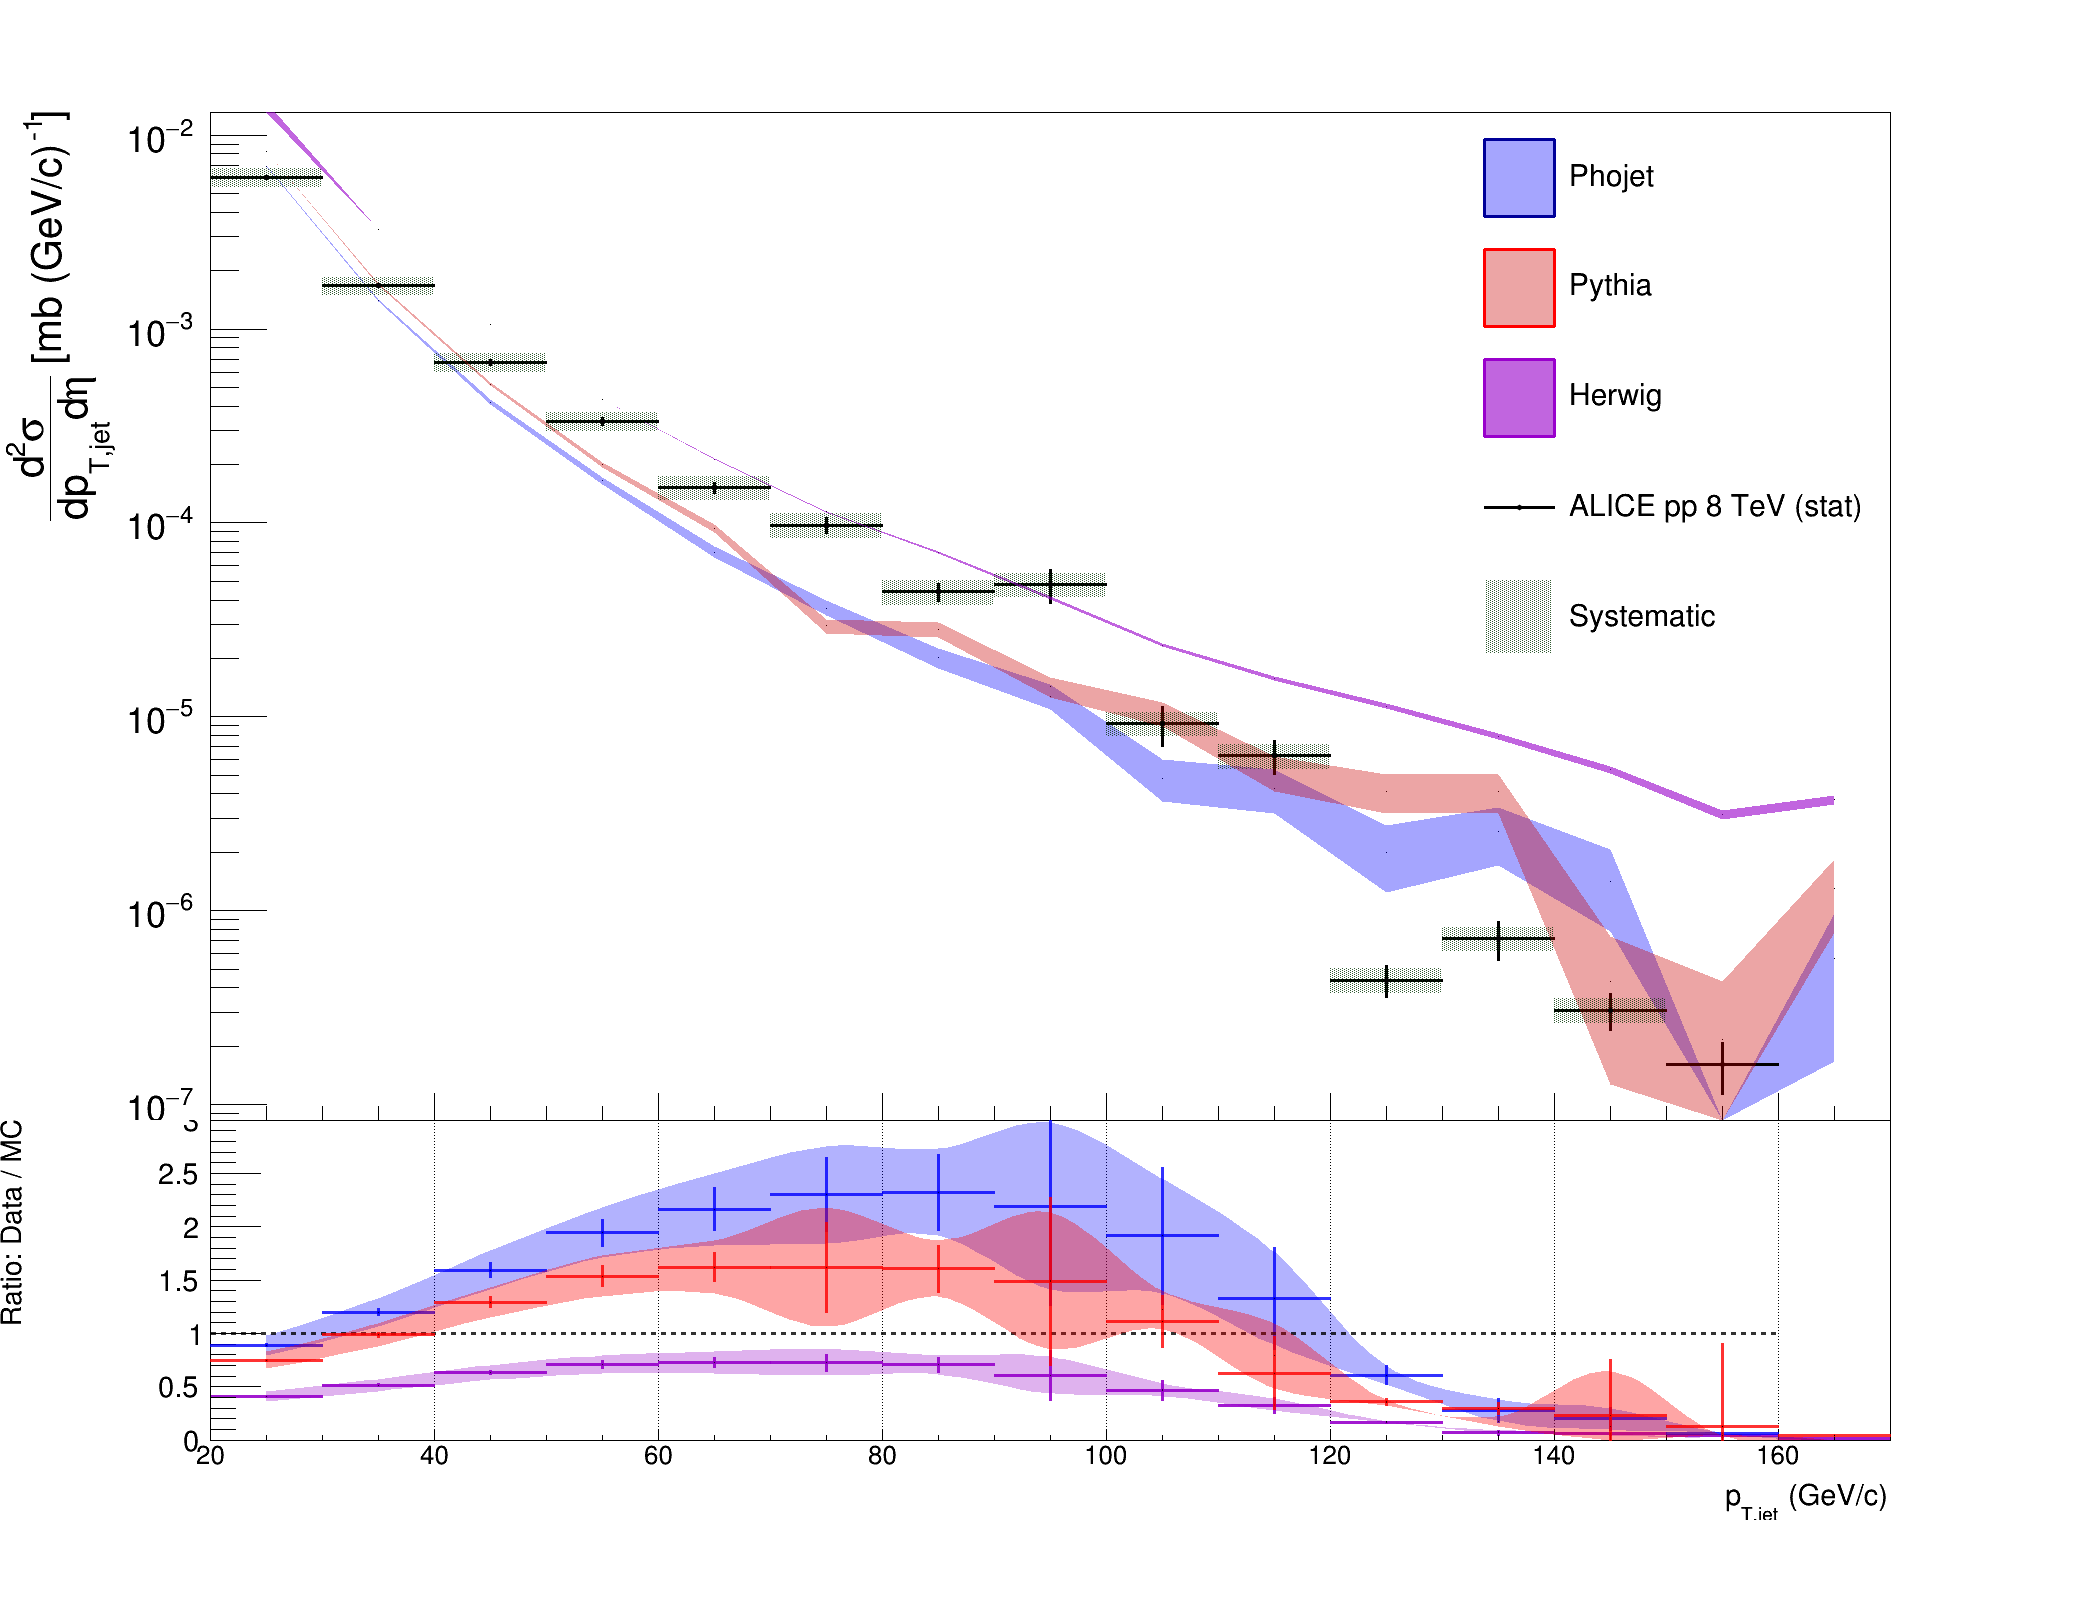
\includegraphics[width=\linewidth]{XSecR04}
\centering
\caption{8 TeV inclusive jet differential cross-section for R = 0.4.}
\label{fig:JetXsecR04}
\end{figure}

\clearpage
}

\noindent
Figures \ref{fig:JetXsecR02}, \ref{fig:JetXsecR03}, and \ref{fig:JetXsecR04} show the inclusive jet cross-sections for radii R = 0.2 through R = 0.4.  The cross-sections incorporate all of the quality assurance criteria, corrections, and uncertainties discussed in the previous chapters.  The figures are split into two sections.  The cross-sections as measured from ALICE along with the associated statistical errors are shown in black.  The associated systematic errors from the ALICE data are shown as the green shaded area.  Min Bias Monte Carlo generated events from PYTHIA, PHOJET, and HERWIG are included and shown as colored solid bands to convey the statistical uncertainties from each simulation.  On the bottom half of each plot are the relative ratios of the ALICE jet cross-sections to one of the Monte Carlos using the same color scheme as above.  

First, we can see that the cross-sections are measured over a wide range, about five orders of magnitude, between 20 GeV/\textit{c} to 160 GeV/\textit{c} in $p_{T}$. The R = 0.2 and R = 0.3 cross-sections show a well defined trend between 20 GeV/\textit{c} - $\sim$100 GeV/c, after this point the data  has a hard drop after which the data points show wider fluctuations.  This same trend is seen in the R = 0.4 jet cross-section but the jerk happens earlier in $p_{T}$ around  80 GeV/\textit{c}.  The fluctuations are an artifact of the bin-by-bin corrections and the lack of EMCal trigger simulations as discussed in Chapter \ref{ch:error}.  

Comparing the results to other CERN experiment is difficult.  ATLAS reported inclusive jet cross-sections from the 8 TeV data for R = 0.4 jets\cite{Aaboud:2017dvo}.  However, ATLAS only performs jet finding down to 100 GeV/\textit{c} and any comparisons are difficult due to the wide statistical fluctuations in the highest-$p_{T}$ bins from ALICE.  A similar issue exists with jet cross-sections reported from CMS at 8 TeV\cite{CMS:2013kda}.  The CMS results report jet cross-sections down to 80 GeV/\textit{c} but only for jets with a radius of R = 0.7.  

Comparing the data to the models we see that the two simulations produced by the ALICE Collaboration, PYTHIA and PHOJET, tend to under predict the data.  PHOJET has the least agreement with the data.  The poor agreement with PHOJET can be explained by the fact that PHOJET is an older Monte Carlo generator and better tuned to describing lower energy experiments.  PHOJET may also be under estimating the data because it focuses on describing photon interactions.  

The Monte Carlo Simulation from HERWIG was produced on a local server farm at the University of Tennessee.  A Min Bias tune of HERWIG was used and 150 million events were generated.  This is reflected in the low statistical errors seen with the HERWIG model compared to either PYTHIA or PHOJET.  The HERWIG simulation tends to slightly over predict the data. 

 Both HERWIG and PYTHIA agree well with the data between 20 GeV/c to 100 GeV/c.  It is hard to say that one is `better' than the other because of the relatively large statistical errors from PYTHIA.  However, for the R = 0.4 jet cross-section we can see that the data seems to trend better towards the clusterization description of hadronization used in HERWIG.  At large jet radii hadronization should be a smaller effect.  The better agreement seen for R = 0.4 jets may be due to HERWIG being better at modeling QCD compared to PYTHIA or PHOJET.

These results help to further our understanding of jets and the QCD pheonmena behind them.  Through scaling these results may serve as a reference for heavy-ion collisions and help to better constrain our understanding of parton energy loss mechanisms in the QGP.  


\subsubsection{Jet Cross-Section Ratios}


\noindent
The ratio of the jet cross-sections as a function of the jet radii is defined as,

\begin{equation}
\mathscr{R} (p_{T}; \, R_{1},R_{2}) = \frac{d\sigma(R_{1}) /d\eta \, dp_{T} }{d\sigma (R_{2}) /d\eta \, dp_{T}},
\label{eq:jetxsecratio}
\end{equation}

\noindent
where $R_{1}$ and $R_{2}$ are the jet radii in question. This probes the transverse structure of jets and is sensitive to QCD hardonization\cite{SOYEZ201159}.  Figures \ref{fig:JetXsecRatioR02}, \ref{fig:JetXsecRatioR03}, and \ref{fig:JetXsecRatioR023} report the ratios of the jet cross-sections between R = 0.2 / R = 0.4, R = 0.3 / R= 0.4, and R = 0.2 / R = 0.3 respectively.  The figures show the relative ratios plotted from the 8 TeV ALICE data, PYTHIA, PHOJET, and HERWIG.  Errors between the cross-sections of different radii were considered uncorrelated.

\afterpage{%

\begin{figure}
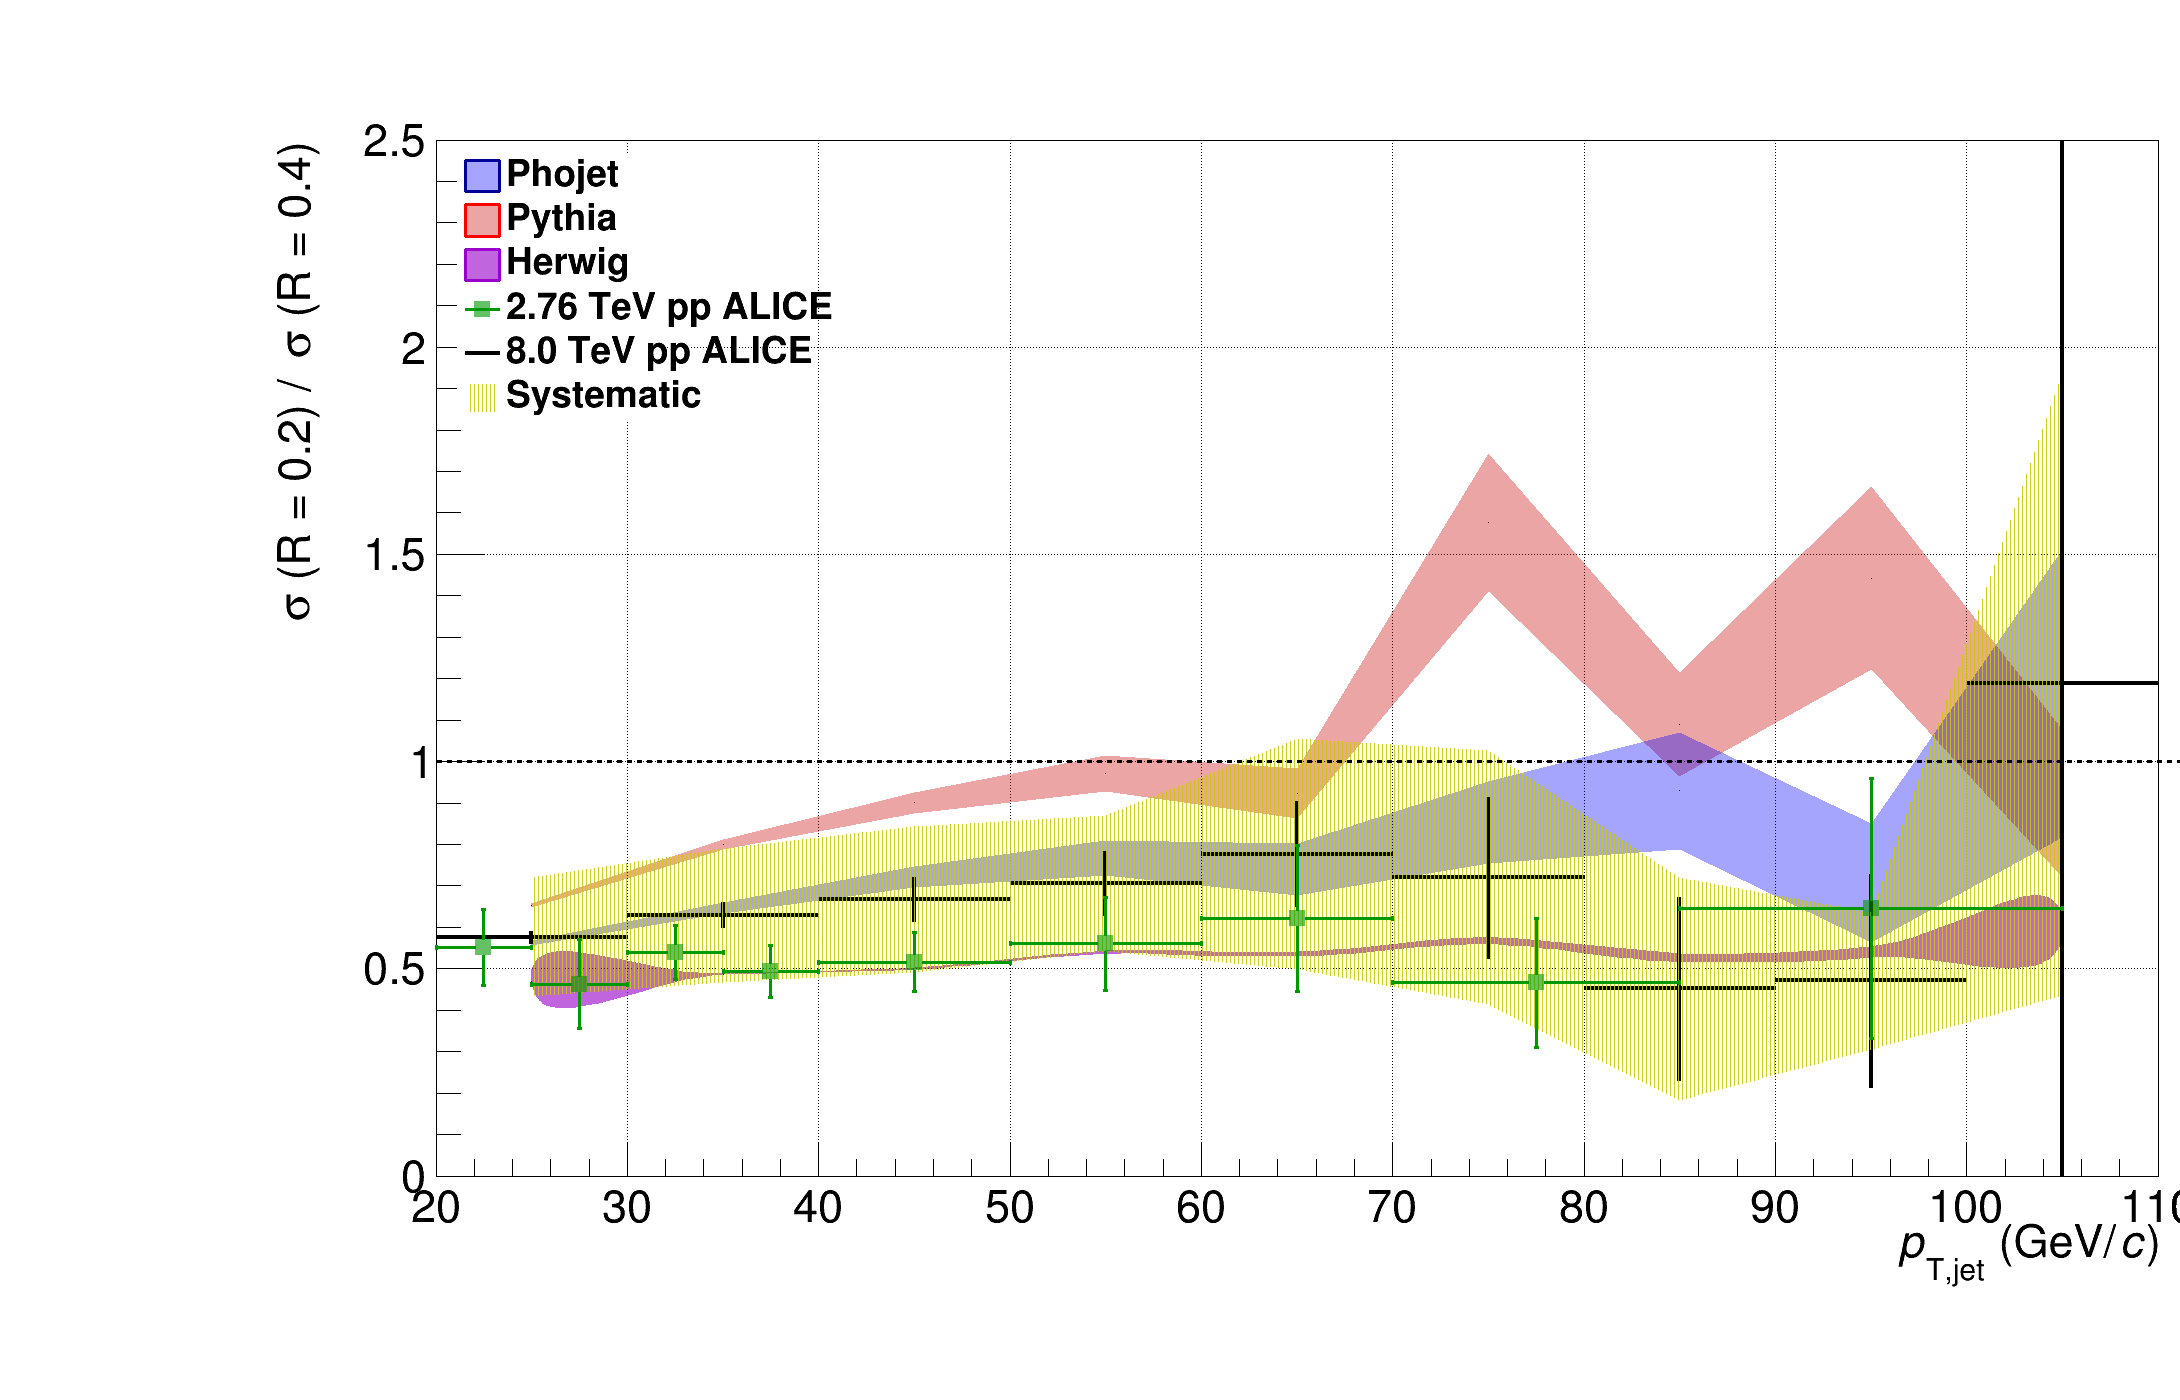
\includegraphics[width=\linewidth]{XSecRatioR02}
\centering
\caption{Ratio of the jet cross-sections R = 0.2  to R = 0.4.}
\label{fig:JetXsecRatioR02}
\end{figure}

\begin{figure}
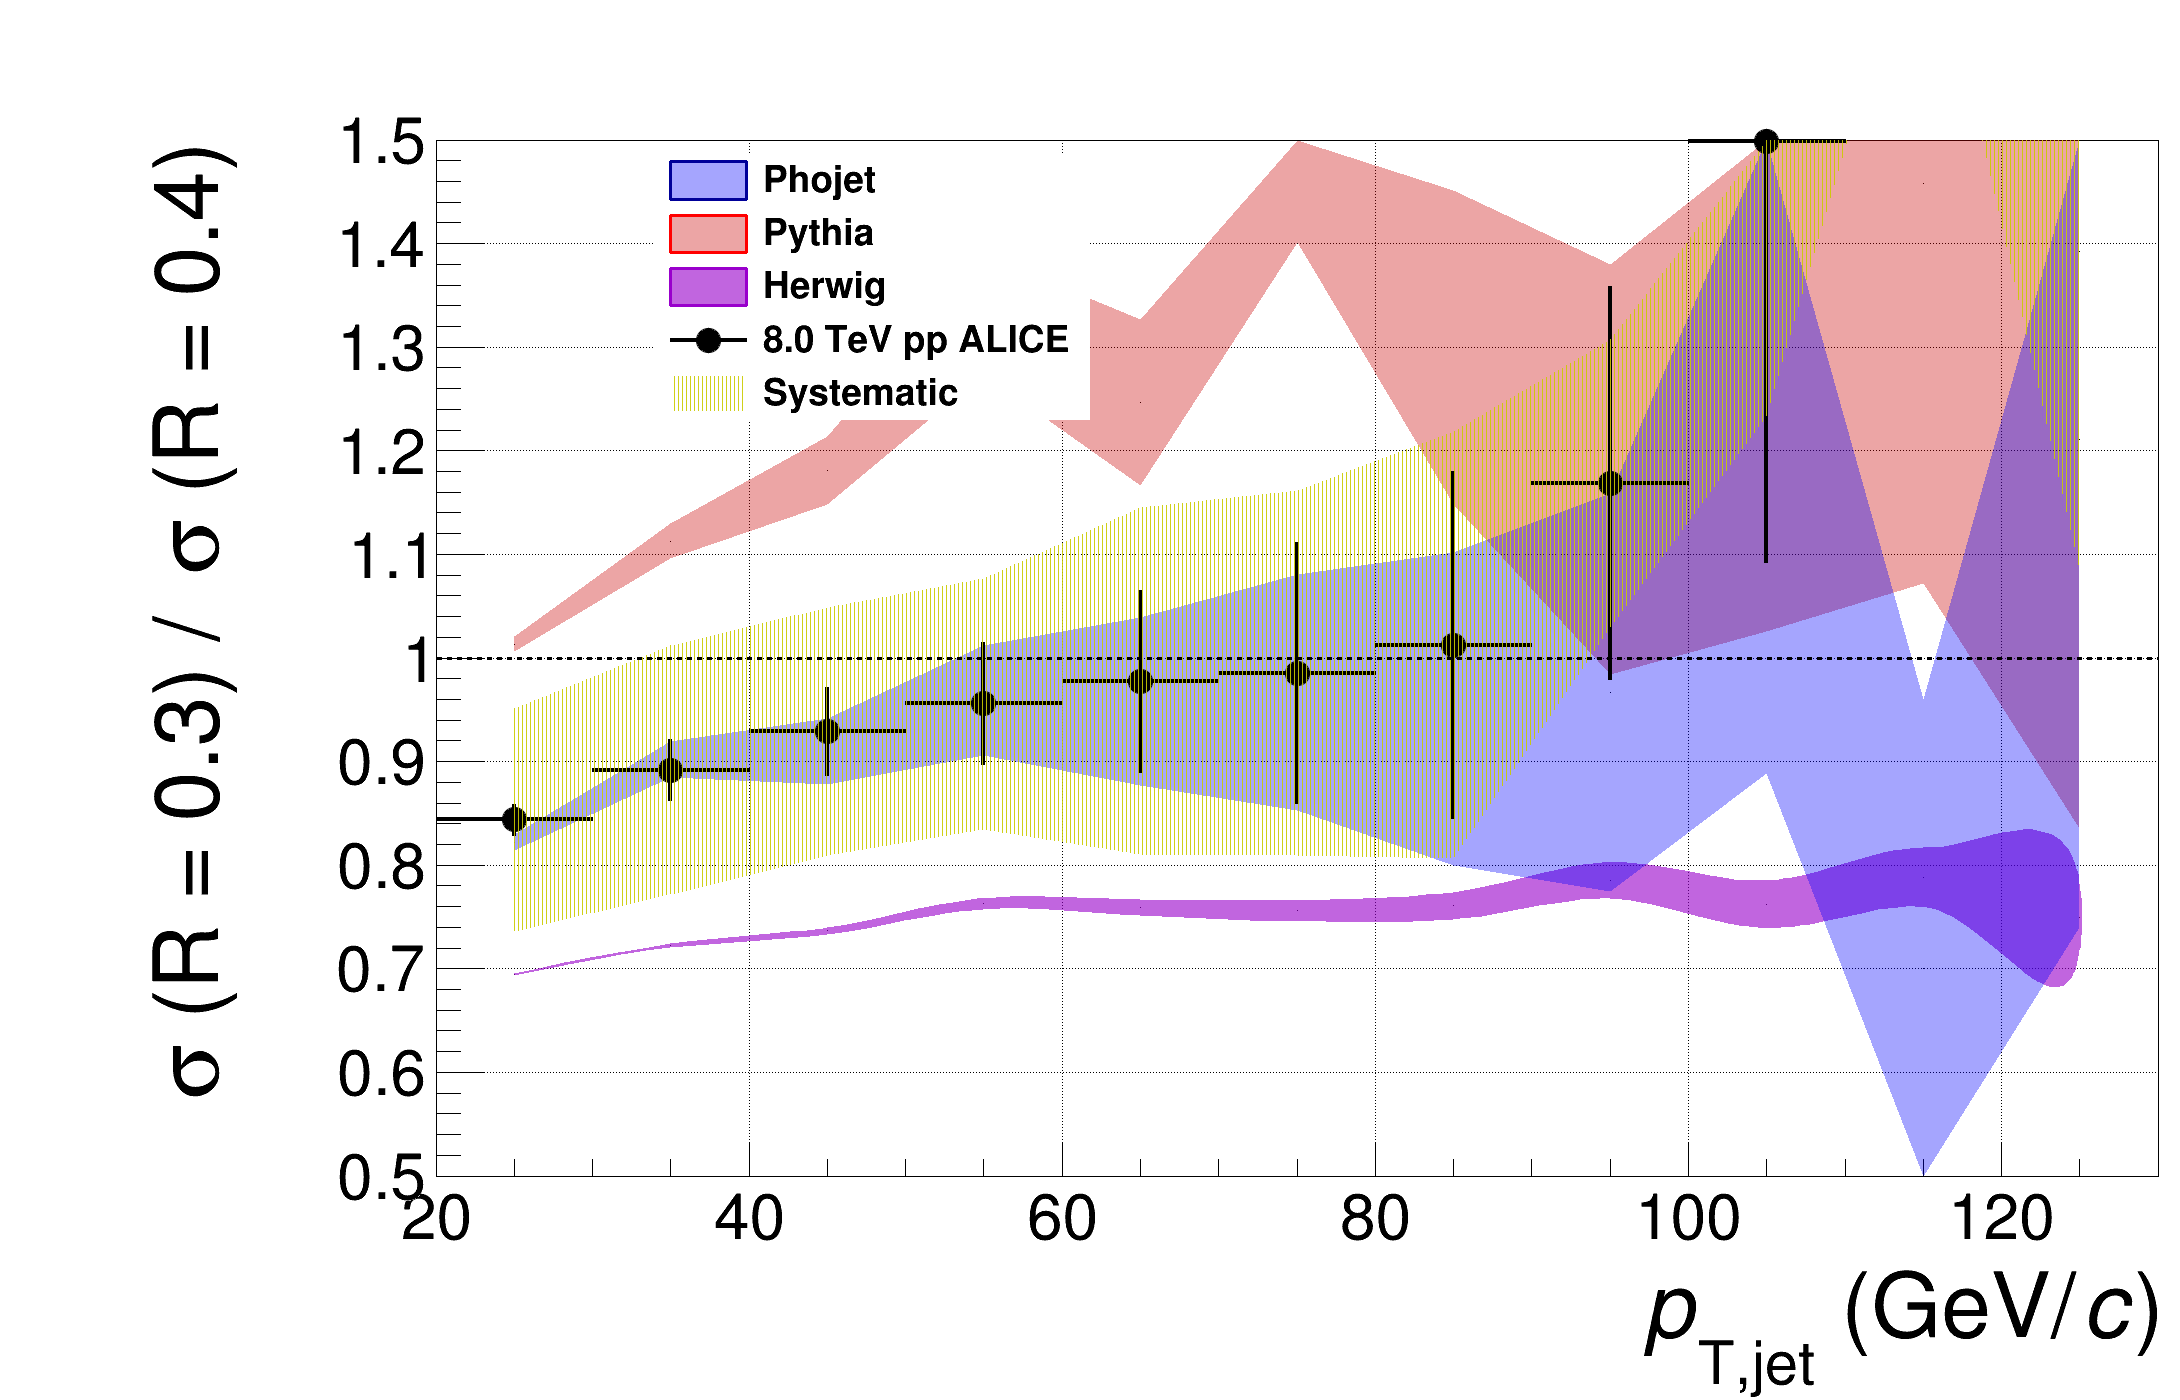
\includegraphics[width=\linewidth]{XSecRatioR03}
\centering
\caption{Ratio of the jet cross-sections R = 0.3  to R = 0.4.}
\label{fig:JetXsecRatioR03}
\end{figure}


\begin{figure}
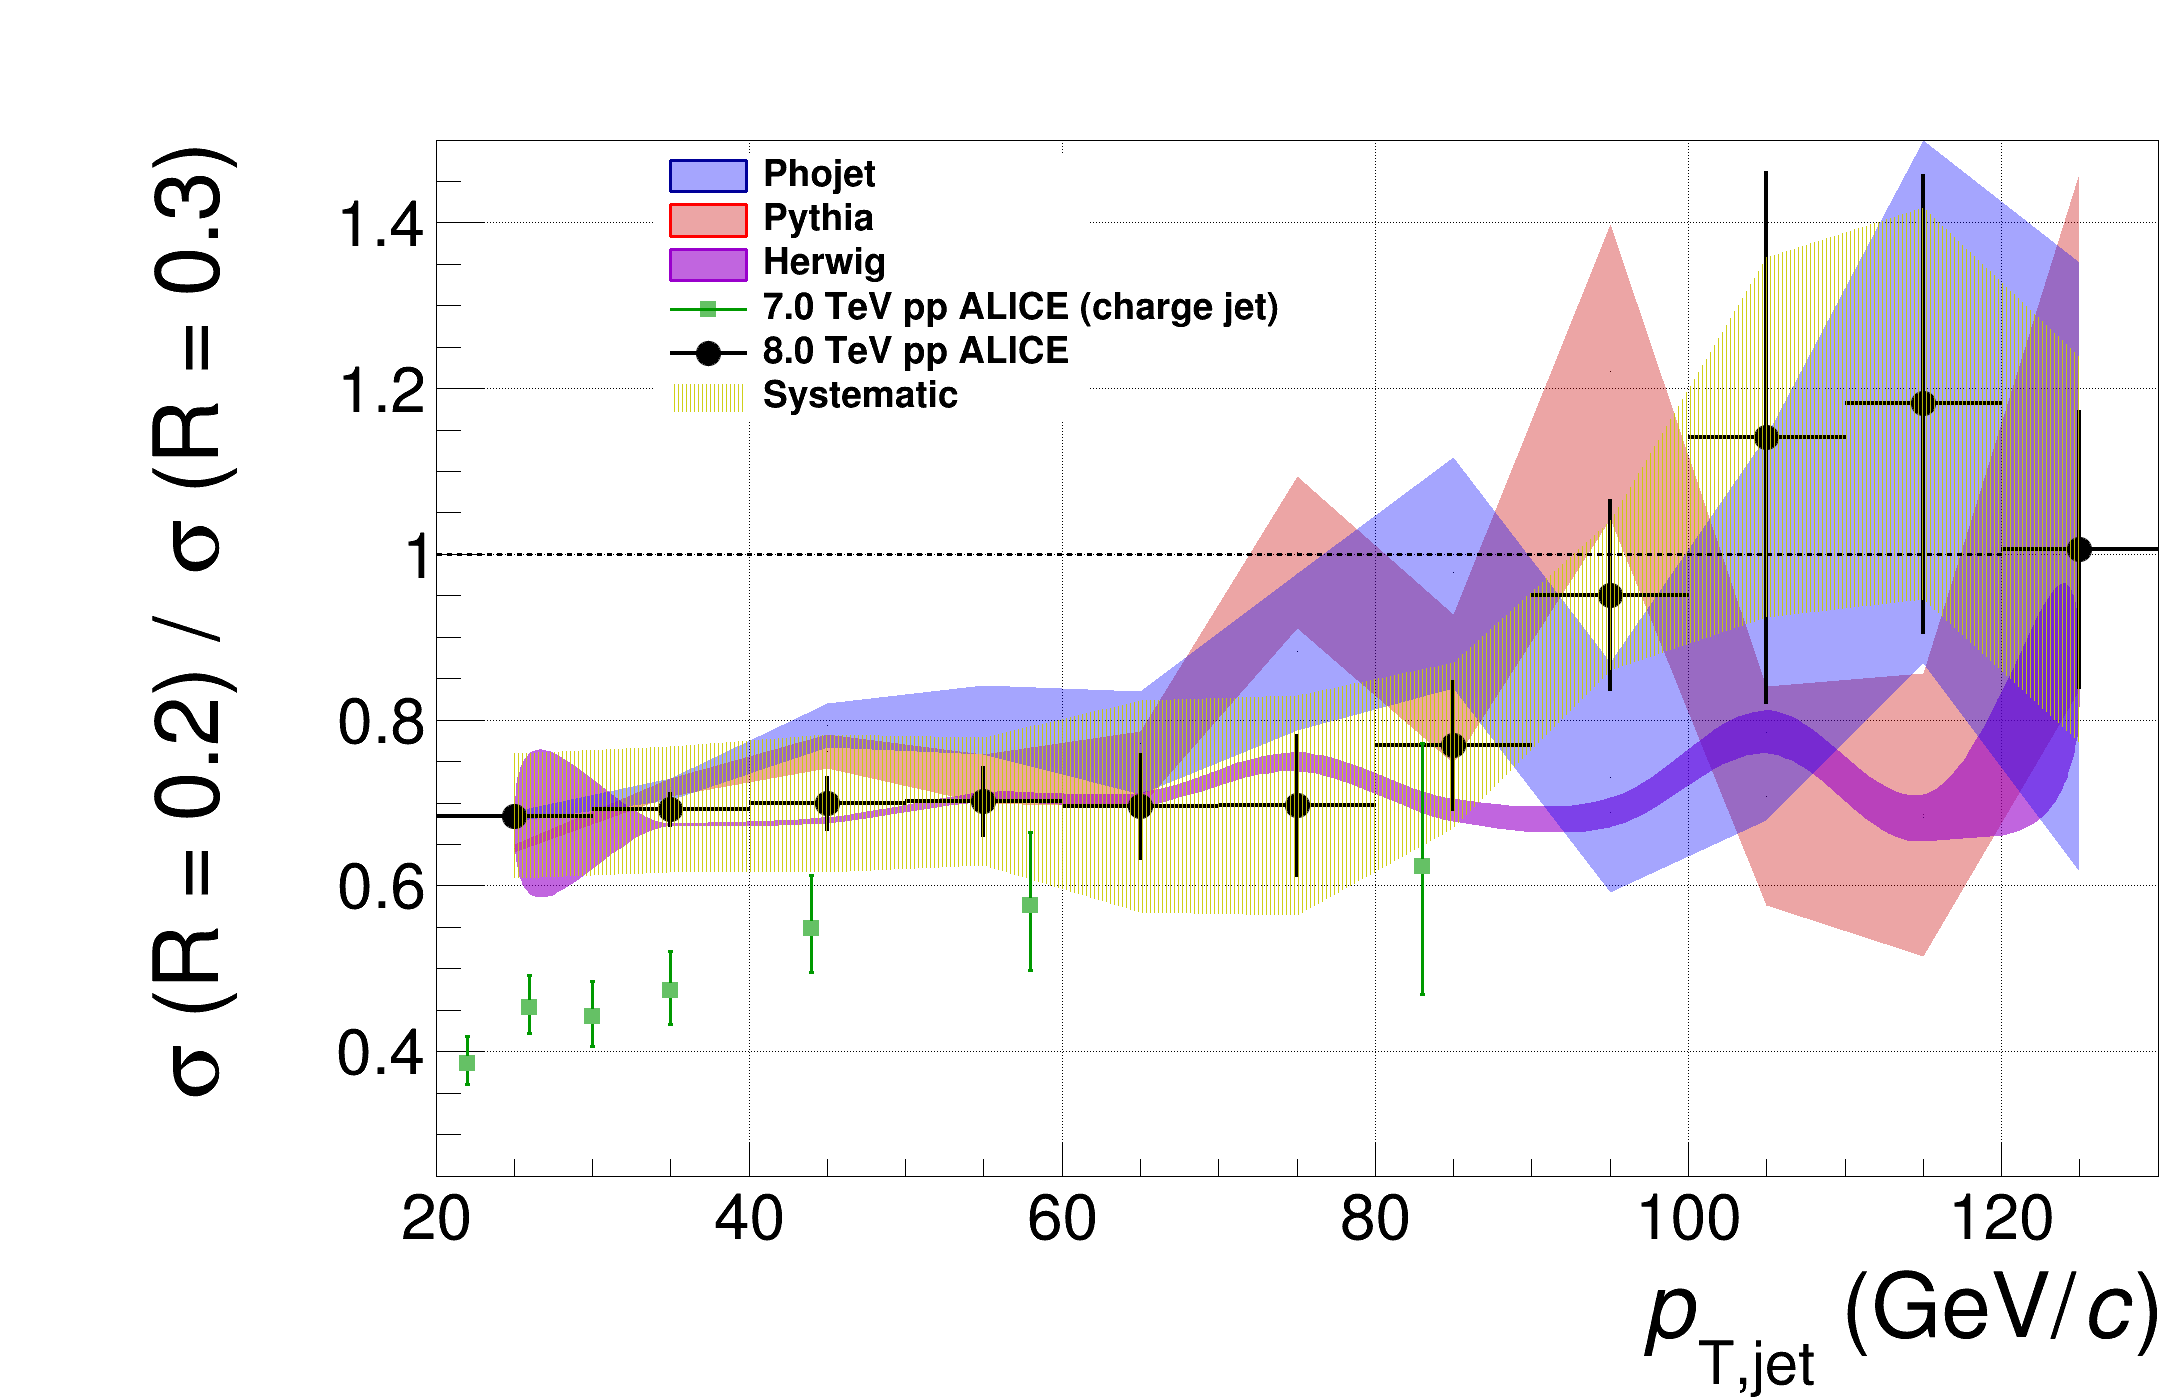
\includegraphics[width=\linewidth]{XSecRatioR023}
\centering
\caption{Ratio of the jet cross-sections R = 0.2  to R = 0.3.}
\label{fig:JetXsecRatioR023}
\end{figure}

\clearpage
}


A similar analysis to this thesis was performed using a 2.76 TeV  data sample collected from ALICE\cite{MA2013319} and it is compared to the 8 TeV data seen in Figure \ref{fig:JetXsecRatioR02} and \ref{fig:JetXsecRatioR023} using green bullet points.  

In order to avoid double counting by sampling the same jet found using different radii parameters in Fastjet I used a disjointed samples of the 8 TeV data to generate each of the ratio plots.  To use the full data set it would be necessary to generate the covariance matrix which is a non-trivial process.   

From the results of the cross-section ratios, we see that the 8 TeV data as reported from this thesis agrees well with the 2.76 TeV results in Figure \ref{fig:JetXsecRatioR02}.  Interestingly it seems that the PHOJET model agrees well with the data for all three figures and is the simulation that agrees the best for the $\sigma (R = 0.3)$ / $\sigma (R = 0.4)$ ratio.  It can be concluded that the PYTHIA ratios have the least agreement because it only includes the LO matrix to calculate partonic showers, which does not model the angular ordering of QCD radiation very well.  HERWIG tends to under predict the data, especially at low-$p_{T}$, which is expected and may be understood in terms of limitations modeling low energy background particles with the tune used in this thesis (v2.3).  

Similar to the previous results these ratios can be used to constrain jet quenching in the QGP.  These results also report the first ratio of jet cross-sections between R = 0.2 and R = 0.3.  This is especially helpful for heavy-ion collisions as most jet results from heavy-ions use either an R = 0.2 or R = 0.3 jet radius to suppress the background in the high multiplicity environment.


\section{Summary and Conclusion}

* - WORK IN PROGRESS - *

Hadronization is the phenomena by which colored partons are confined to colorless hadrons.  When two partons undergo a high energy collision they will fragment and hadronize into a jet.  By measuring jet properties in proton-proton collisions we can probe different hadronization models.  In heavy-ion collisions a new form of matter known as the Quark-Gluon Plasma is created.  Jets are created at the earliest moments of a heavy-ion collision and are sensitive to energy loss mechanisms in the QGP.  Reconstructing full jets in proton-proton collisons serves as a baseline measurement for understanding jet quenching in the QGP. 

This thesis presents the first measurements of inclusive full jets at $\sqrt{s} = \,$ 8 TeV using the ALICE detector.  Using the time projection chamber and the electromagnetic calorimeter one may obtain a satisfactory level of uncertainty to both the jet energy scale and jet yields.  In addition, a novel approach to reconstruct the jet that fired the high-$p_{T}$ EMCal trigger and scale this in order to combine with Min Bias events.  By combing the two triggered data samples we obtained jet measurements over a wide kinematic range, especially to low momentum.  Low-momentum reconstruction of jets and their constituents probe jet quenching in heavy-ion collisions.

The good agreement between the 8 TeV data and Monte Carlo simulations show the jets are a well calibrated probe for testing QCD phenomena.  In terms of the kinematic reach, the results of this thesis are in good agreement with QCD calculations down to 20 GeV/\textit{c} through 100 GeV/\textit{c} in $p_{T}$.  This range may be extended with better Monte Carlos in the future.  With better Monte Carlo simulations we could see the range extend to 200 GeV/\textit{c} in $p_{T}$ using the EMCal triggered data.  The comparisons between the data and the model predictions agree well, with the most tension lying with PHOJET.  

The results from this thesis can also be used in future heavy-ion runs to probe jet quenching, as these results would serve as a baseline comparison.   Scaling down the obtained cross-sections to energies at which lead-lead collisions are currently performed allows for the determination of the nuclear modification factor.  The work in this thesis also presents the jet measurements from ALICE down to 20 GeV/\textit{c}, which will be important for probing energy loss in the QGP.  By measuring these very low energy jets we can probe the full kinematic range and energy loss mechanism for jets.  Previous higher energy jet results would tend to bias to jets to those that traveled a short distance through the QGP.

In addition to the jet results, this thesis presented work upgrading the ALICE TPC in anticipation for the high luminosity upgrade of the LHC scheduled to begin in mid-2021.  The multiwire proportional chamber design of the original TPC will be replaced with a stack of gaseous electron multiplier foils that will allow for a continuous readout of data.

With the increase in energy and luminosity seen at the LHC, we have moved into the era of high-precision testing of pQCD.  The work set forward by this thesis sets the stage for using jets with ALICE data in the future, especially after the high luminosity upgrade of the LHC is complete.  Although it dates to 2012, the 8 TeV contains some of the largest data samples available at a given energy from the LHC.  This makes it an important data set and worthy of future investigations.  What results we will gain from the upgraded LHC and jets is only left to our imagination and to nature's mercy.



* - WORK IN PROGRESS - *